\documentclass[12pt]{article}
\usepackage{amsmath}
\usepackage{amssymb}
\usepackage{enumitem}
\usepackage{graphicx}
\usepackage{hyperref}
\usepackage{tikz}

\title{CS461 Homework 3}
\author{Mannan Shukla}
\date{Due: Nov. 19, 11:59 PM}

\begin{document}

\maketitle

\section*{1. Decision Tree}
\section*{1.1 Information Gain and Root Node Selection}

The initial entropy of the $\text{Play}$ is: $H(Play) = 1.0000$

\begin{itemize}
    \item \textbf{Weather:} $IG(\text{Weather}) = 0.4000$
    \item \textbf{Temperature:} $IG(\text{Temperature}) = 0.1145$
    \item \textbf{Humidity:} $IG(\text{Humidity}) = 0.0349$
    \item \textbf{Wind:} $IG(\text{Wind}) = 0.1245$
\end{itemize}

\noindent Since \textbf{Weather} has the highest Information Gain $0.4000$, it is selected as the root node of the decision tree.

\begin{center}
    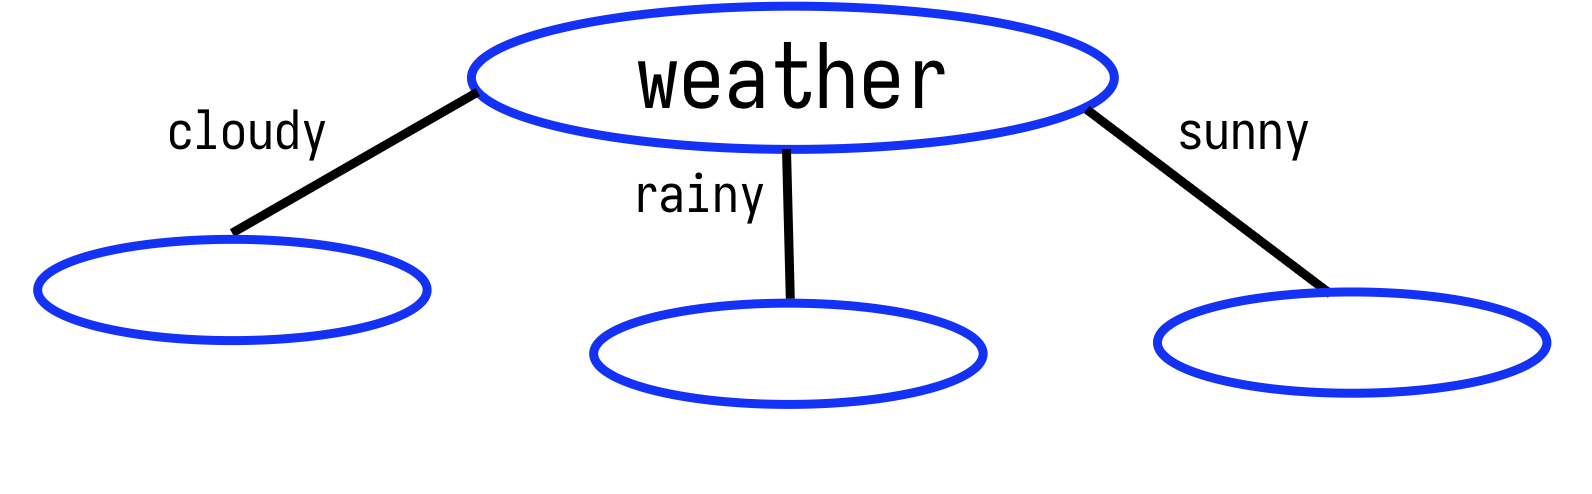
\includegraphics[width=0.8\textwidth]{1.png}
\end{center}

\section*{1.2 Constructing the Decision Tree}

The decision tree is shown below:

\begin{center}
    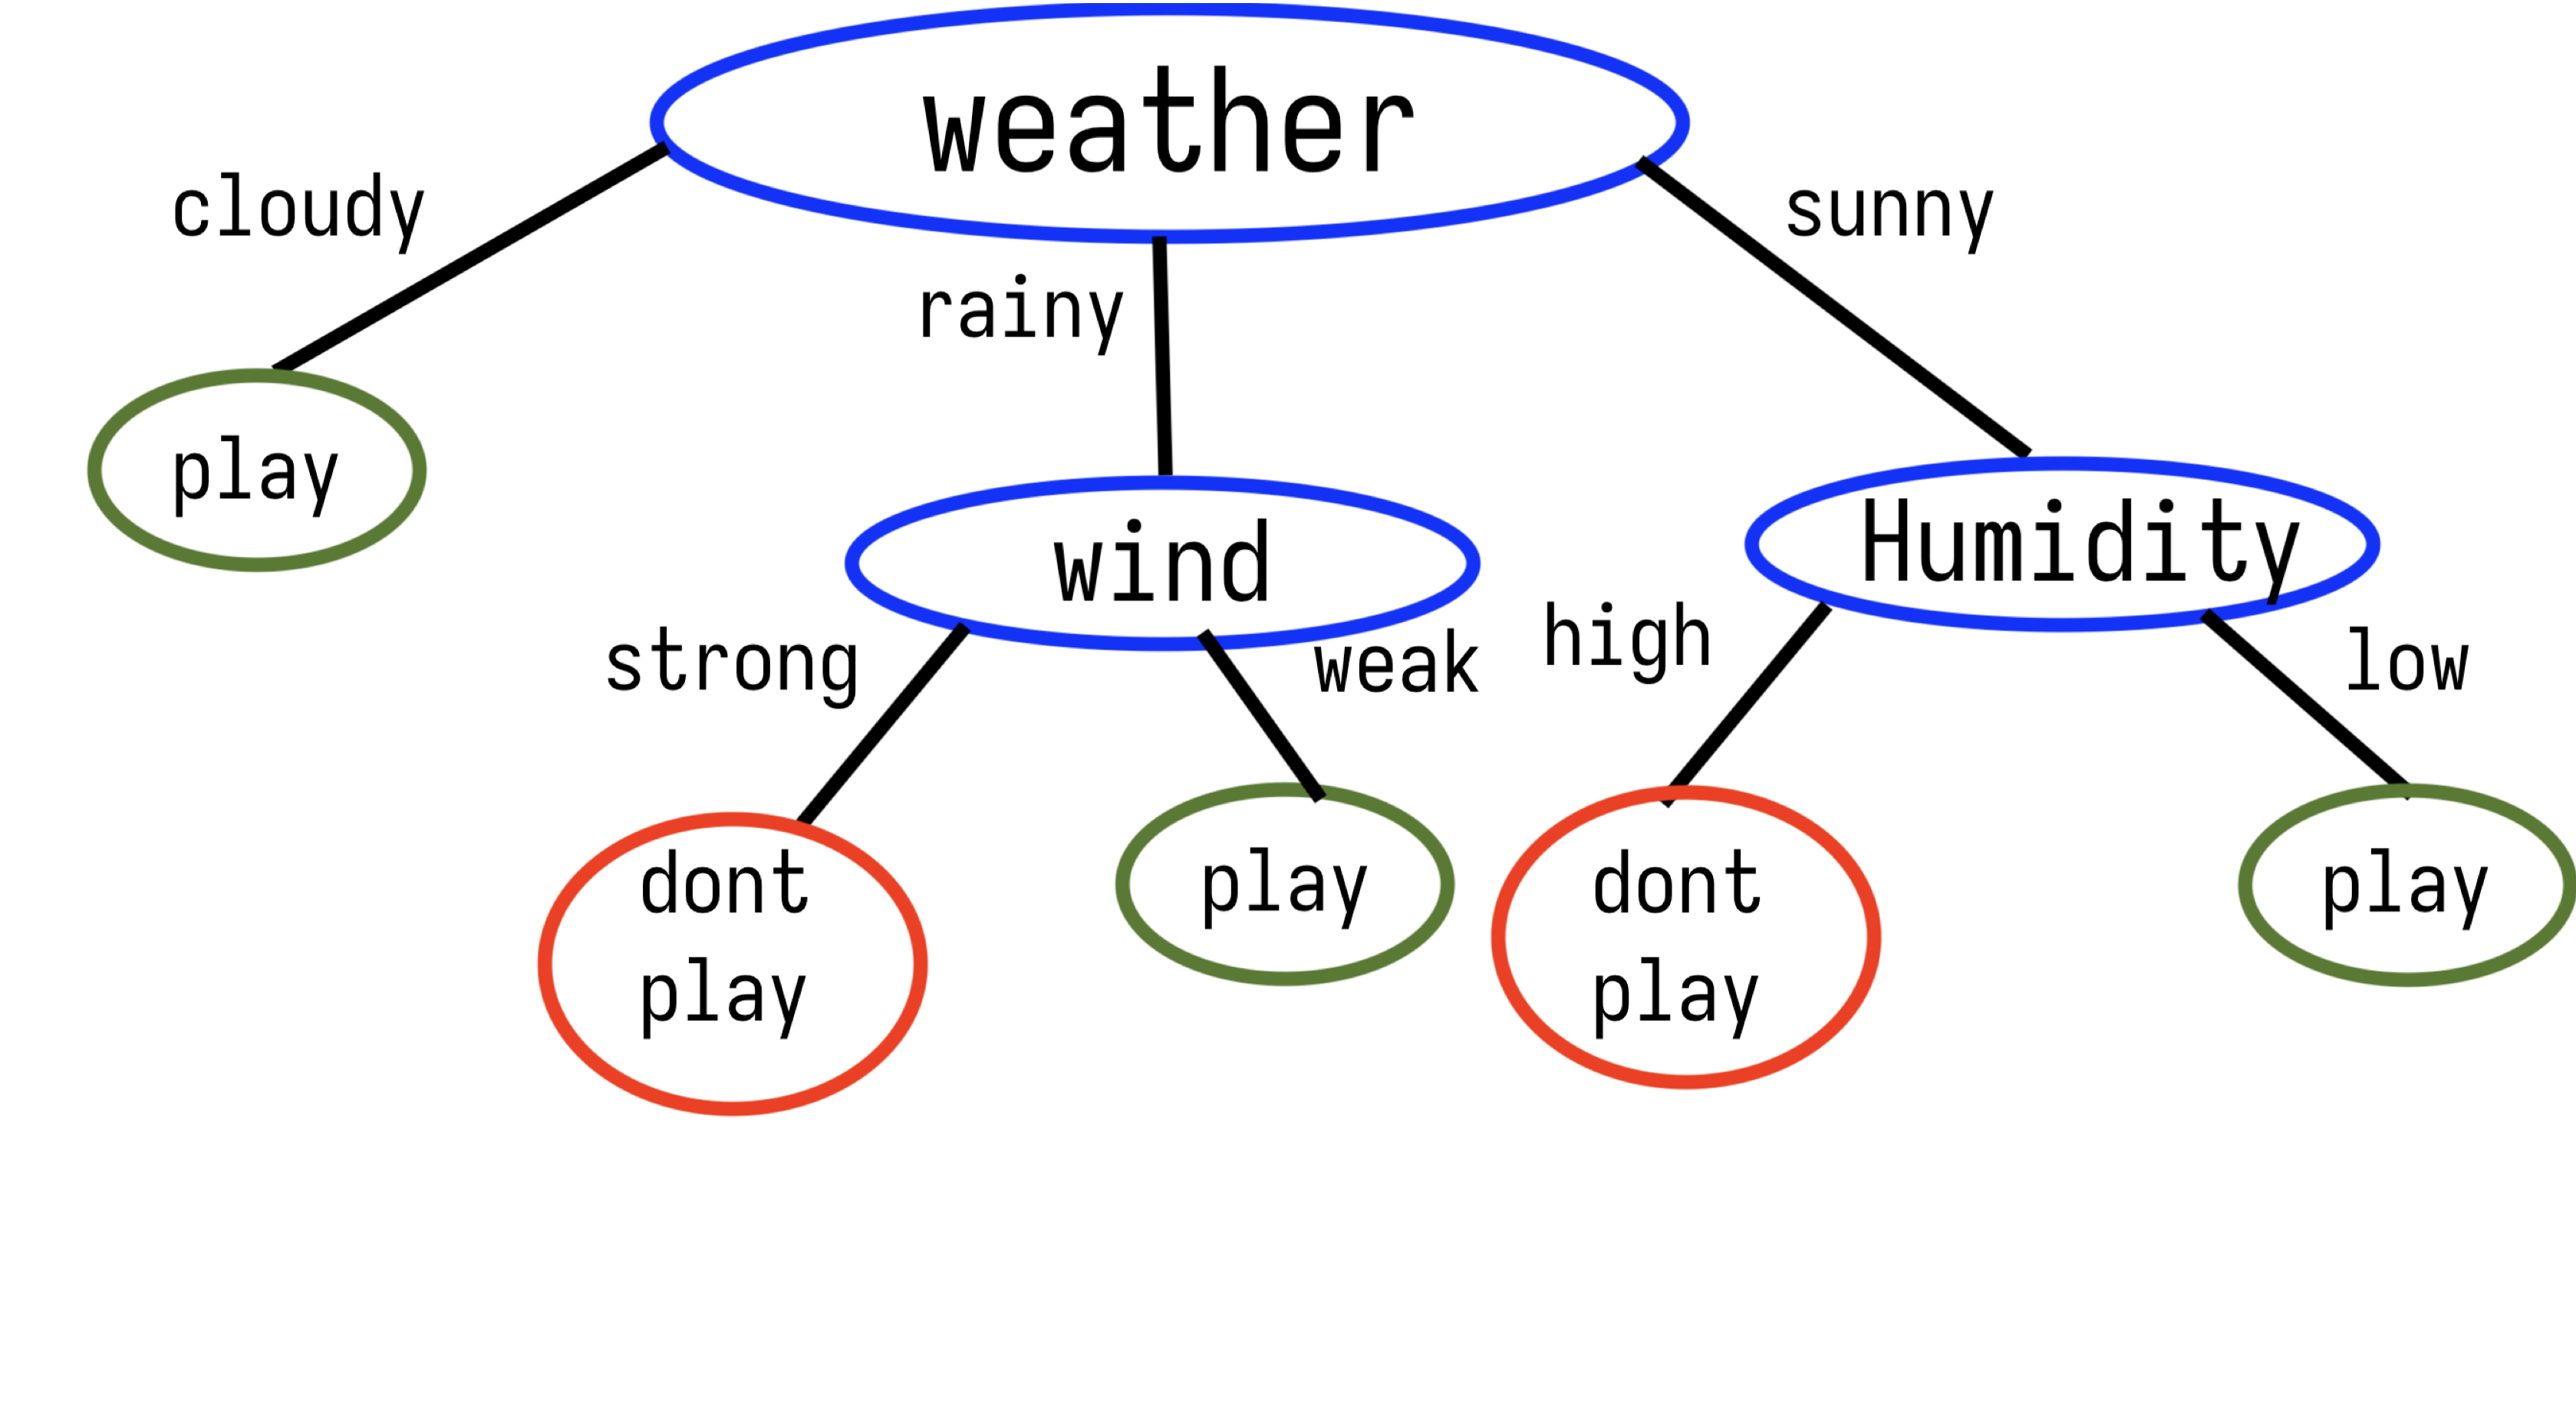
\includegraphics[width=0.8\textwidth]{2.png}
\end{center}

\subsection*{1.3 Pruning (Extra Points)}

\[
C(T) = \sum_{\tau \in T'} Q(\tau) + \lambda \cdot \text{num of leaves in } T'
\]

For the initial tree:
\[
C(T) = 0 + \lambda \cdot 5 = 5\lambda
\]

When pruning the \textbf{Humidity sub-tree}:
\[
C(T) = - \left( \frac{1}{3} \log_2 \frac{1}{3} + \frac{2}{3} \log_2 \frac{2}{3} \right) + \lambda \cdot 4
\]
\[
C(T) = 0.918 + \lambda \cdot 4
\]

When pruning the \textbf{Wind sub-tree}:
\[
C(T) = - \left( \frac{1}{4} \log_2 \frac{27}{256} \right) + \lambda \cdot 4
\]
\[
C(T) = 0.811 + \lambda \cdot 4
\]

Pruning to the \textbf{root only}:
\[
C(T) = - \left( \frac{5}{10} \log_2 \frac{5}{10} + \frac{5}{10} \log_2 \frac{5}{10} \right) + \lambda \cdot 1
\]
\[
C(T) = 1 + \lambda
\]

\textbf{Observation:} As \( \lambda \) increases, the penalty for the number of leaves grows. At \( \lambda = 0 \), the unpruned tree minimizes cost. For \( \lambda = 0.25 \), pruning to the root achieves the lowest cost.

\section*{2. Perceptron}
\subsection*{2.1 Single Data Point}
With a step size of $1$, it will always take $\textbb{one}$ iteration to classify the data point.

\subsection*{2.2 Random Initialization}

Given a randomly initialized weight vector, if $w_0$ correctly classifies the point, then $0$ iterations will be required, otherwise, we must consider another case: 

Let \(w_0 = (a_1, a_2) \neq (0, 0)\). If \(a_1x_1 + a_2x_2 > 0\), then the point is classified correctly without requiring any updates. If \(a_1x_1 + a_2x_2 \leq 0\), first define \(x = (x_1, x_2)\).

We claim that for all \(n \in \mathbb{N}\), the weight vector after \(n\) iterations is given by \(w_n = w_0 + n x\). To prove this, note that for \(n = 1\), we have \(w_1 = w_0 + x\) by the definition of the Perceptron update rule. For a fixed \(n = k\), assume \(w_k = w_0 + kx\). Then, for the next iteration:
\[
w_{k+1} = w_k + x = (w_0 + kx) + x = w_0 + (k + 1)x.
\]

By induction, \(w_n = w_0 + nx\) holds for all \(n \in \mathbb{N}\).

For the classifier to correctly classify the point \(x\), we require \(w_n \cdot x > 0\), where:
\[
w_n \cdot x = (w_0 + nx) \cdot x = w_0 \cdot x + n \|x\|^2.
\]

Since \(\|x\|^2 = x_1^2 + x_2^2 > 0\) and \(w_0 \cdot x = a_1x_1 + a_2x_2 \leq 0\) by assumption, we have:
\[
w_n \cdot x > 0 \implies n > -\frac{w_0 \cdot x}{\|x\|^2}.
\]

Thus, choose \(n \in \mathbb{N}\) such that \(n > -\frac{w_0 \cdot x}{\|x\|^2}\). This is the number of iterations required for the Perceptron to correctly classify the data point if it was initially misclassified.

\subsection*{2.3 Iterative Updates}

\[
\begin{array}{|c|c|}
\hline
\textbf{Iteration} & \mathbf{w} \\ \hline
0 & w_0 = (0, 0) \\ \hline
1 & w_1 = (0, 0) + (0, 1) = (0, 1) \\ \hline
2 & w_2 = (0, 1) - (1, 0.5) = (-1, -0.5) \\ \hline
3 & w_3 = (-1, -0.5) + (1, 1) = (0, 1.5) \\ \hline
4 & w_4 = (0, 1.5) - (1, 0.5) = (-1, 1) \\ \hline
5 & w_5 = (-1, 1) + (1, 1) = (0, 2) \\ \hline
6 & w_6 = (0, 2) - (1, 0.5) = (-1, 1.5) \\ \hline
\end{array}
\]

\section*{3. Gaussian Discriminant Analysis (GDA)}

\subsection*{3.1 Estimating Parameters}
\begin{table}[h!]
\centering
\begin{tabular}{|c|c|c|}
\hline
\textbf{Class} & \textbf{Mean (\(\mu\))} & \textbf{Variance (\(\sigma^2\))} \\ \hline
Class +1       & -0.0722                 & 1.3031                          \\ \hline
Class -1       & 0.9402                  & 1.9426                          \\ \hline
\end{tabular}
\caption{Mean and variance for each class.}
\label{tab:class_stats}
\end{table}

\subsection*{3.2 Test Accuracy}
The test accuracy is 61\%

\subsection*{3.3 Improving the Classifier}
As currently constructed, we use MLE estimation. MLE only looks at likelihood and ignores prior probabilities. Using MAP rule, we can increase our effectiveness. With MAP, accuracy went up to 90\%

\subsection*{3.4 2D GDA Statistics}
Table is on the next page

\begin{table}[h!]
\centering
\begin{tabular}{|c|c|c|}
\hline
\textbf{Class} & \textbf{Mean (\(\mu\))} & \textbf{Covariance (\(\Sigma\))} \\ \hline
Class +1       & \([0.0130754, 0.06295251]\) & 
\(\begin{bmatrix}
0.98285498 & 0.00612046 \\ 
0.00612046 & 1.05782804 
\end{bmatrix}\) \\ \hline
Class -1       & \([-0.02313942, -0.02114952]\) & 
\(\begin{bmatrix}
1.00329037 & -0.01142356 \\ 
-0.01142356 & 4.97693356 
\end{bmatrix}\) \\ \hline
\end{tabular}
\caption{3.4 - Mean and covariance for each class.}
\label{tab:class_stats}
\end{table}

\subsection*{3.5 2D GDA Predictions}
The test accuracy is 84\%

\subsection*{3.6 Density-Based Accuracy (Extra Points)}
The test accuracy is 85\% which shows us that GDA is suitable. GDA provides a reasonable framework for classification because it balances robustness, simplicity, and efficiency, achieving near-optimal accuracy even when the data deviates slightly from Gaussian assumptions. A more complex mixture model wasn't that much of an improvement.

\section*{4. Logistic Regression}
\subsection*{4.1 Data Preprocessing}

TF-IDF is a weighted metric that finds words that best describe one and only one document from a corpus of documents. It finds the frequency of the word in the document, then weights frequency outside of the target document negatively, making sure there is a degree of uniqueness to the word and the document.

\subsection*{4.2 Dimensionality Reduction}
file is attached

\subsection*{4.3 Gradient Descent}
file is attached

\subsection*{4.4 Train and Test Accuracy}
Train Accuracy: 97.03\%
Test Accuracy: 0.96\%

\subsection*{4.5 Extra Points: Email Classification}

\end{document}
